\documentclass[xcolor=table]{beamer}

\mode<presentation> {
  \usetheme{CambridgeUS}
}
\usecolortheme{seahorse}
\setbeamertemplate{navigation symbols}{}

\usepackage{graphicx} % Allows including images
\usepackage{booktabs} % Allows the use of \toprule, \midrule and \bottomrule in tables

\usepackage[utf8]{inputenc}
\usepackage[T2A]{fontenc}
\usepackage[english,russian]{babel}
\usepackage{listings}
\usepackage{xcolor}
\usepackage{caption}
\usepackage{stmaryrd}



\usepackage{biblatex}

\bibliography{main.bib}

\newcommand{\citepres}[1]{{\it \citetitle{#1}}, \citeauthor{#1}, \citeyear{#1}}

\renewcommand{\footnotesize}{\tiny}

\title[Университет ИТМО]{Применение метода суперкомпиляции для специализации реляционных программ}

\author{Мария Куклина, M4236}
\institute[ITMO]
{
Университет ИТМО\\ 

Научный консультант: Вербицкая Екатерина Андреевна
\medskip
}
\date{}


\begin{document}

\begin{frame}
\titlepage
\end{frame}

%
% TODO: footnote цвет более серый

%%%%%%%%%%%%%%%%%%%%%%%%%%%%%%%%%%%%%%%%%%%%%%%%%%%
%
%
%%%%%%%%%%%%%%%%%%%%%%%%%%%%%%%%%%%%%%%%%%%%%%%%%%%
\begin{frame}{Реляционное программирование}
\begin{block}{Определение}
    Вид декларативного программирования, в котором программы представляются как набор отношений между аргументами.
\end{block}
\begin{block}{Пример}
  Пример {\it запросов} для отношения умножения $\text{mul}^o \subseteq \text{Int} \times \text{Int} \times \text{Int}$:
  \begin{itemize}
    \item $\texttt{mul}^o(\texttt{2, 2, 4})$ --- проверка корректности отношения.
    \item $\texttt{mul}^o(\texttt{2, 2, C})$ --- поиск всех \texttt{С}, таких что \texttt{2 * 2 = C}.
    \item $\texttt{mul}^o(\texttt{A, 1, 4})$ --- поиск всех \texttt{A}, таких что \texttt{A * 1 = 1}.
    \item $\texttt{mul}^o(\texttt{A, B, C})$ --- поиск всех троек \texttt{A, B, С}, таких что \texttt{A * B = C}.
  \end{itemize}
\end{block}
\end{frame}
%%%%%%%%%%%%%%%%%%%%%%%%%%%%%%%%%%%%%%%%%%%%%%%%%%%
%
%
%%%%%%%%%%%%%%%%%%%%%%%%%%%%%%%%%%%%%%%%%%%%%%%%%%%
\begin{frame}{miniKanren}
  \begin{block}{}
    Встраиваемый предметно-ориентированный язык реляционного программирования\footnotemark.
    % Сказать про логическое программирование в ограничениях
  \end{block}\footnotetext{\citepres{byrdMK}}

  {\bf Применение}
  \begin{itemize}
  \item Замена тяжеловесной подсистемы Prolog для ряда задач.
  \item Генерация программ по спецификации входов и выходов на основе \emph{реляционного интерпретатора}.
  \item Порождение решения задач поиска по решению задачи распознавания\footnote{\citepres{lozov}}.
  \item Поиск лечения редких генетических заболеваний в точной медицине\footnote{\citepres{medMK}}.
  \end{itemize}
\end{frame}
%%%%%%%%%%%%%%%%%%%%%%%%%%%%%%%%%%%%%%%%%%%%%%%%%%%
%
%
%%%%%%%%%%%%%%%%%%%%%%%%%%%%%%%%%%%%%%%%%%%%%%%%%%%
\begin{frame}{Постановка проблемы}

\begin{itemize}
\item Сложные алгоритмы в miniKanren работают медленно.
\item Многие отношения на деле являются функциональными,
  из-за чего запуск в ``обратном'' направлении очень неэффективен.\\
  {\bf Примеры}
  \begin{itemize}
  \item Программы, порождённые инструментом по трансляции из функционального языка в miniKanren\footnote{\citepres{trconv}}.
  \item Порождение решения задач поиска.
  \end{itemize}
\end{itemize}
\end{frame}
%%%%%%%%%%%%%%%%%%%%%%%%%%%%%%%%%%%%%%%%%%%%%%%%%%%
%
%%%%%%%%%%%%%%%%%%%%%%%%%%%%%%%%%%%%%%%%%%%%%%%%%%%
\begin{frame}{Специализация}
\begin{block}{Определение}
Автоматизированная техника оптимизации программ, при которой из программы удаляются
избыточные вычисления, зависимые от частично известного входа\footnotemark.
\end{block}\footnotetext{\citepres{jones}}

\begin{itemize}
\item Частичная дедукция --- класс методов специализации для логический языков, в частности, для Prolog.\footnote{\citepres{advanced}}
\item Специализация miniKanren на основе \emph{конъюнктивной частичной дедукции (CPD)}\footnote{\citepres{lozov}}.
\begin{itemize}
\item Сложна в поддержке, даёт нестабильные результаты.
\item Однако предоставляет библиотеку для построения специализаторов.
\end{itemize}
\end{itemize}
\end{frame}
%%%%%%%%%%%%%%%%%%%%%%%%%%%%%%%%%%%%%%%%%%%%%%%%%%%
%
%%%%%%%%%%%%%%%%%%%%%%%%%%%%%%%%%%%%%%%%%%%%%%%%%%%
\begin{frame}{Суперкомпиляция}

\begin{block}{Определение}
Техника автоматической трансформации и анализа программ, при которой
программа символьно исполняется с сохранением истории вычислений, на основе
которой принимаются решения о трансформации и оптимизации.
\end{block}

\begin{itemize}
\item Суперкомпиляторы применяются во основном для функциональных языков.
\item Суперкомпиляция показывает хорошие результаты при специализации.
\item Полуавтоматическая позитивная суперкомпиляция для Prolog\footnote{\citepres{apropos}}.
\end{itemize}

\end{frame}
%%%%%%%%%%%%%%%%%%%%%%%%%%%%%%%%%%%%%%%%%%%%%%%%%%%
%
%
%%%%%%%%%%%%%%%%%%%%%%%%%%%%%%%%%%%%%%%%%%%%%%%%%%%
\begin{frame}{Цели и задачи}
\begin{block}{Цель}
Улучшение результатов специализации реляционных программ путём применения метода суперкомпиляции.
\end{block}
%%%%%%%%%%%%%%%%%%%%%%%%%%%%%%%%%%%%%%%%%%%%%%%%%%%
%
%
%%%%%%%%%%%%%%%%%%%%%%%%%%%%%%%%%%%%%%%%%%%%%%%%%%%
\begin{block}{Задачи}
\begin{itemize}
\item Реализовать базовый суперкомпилятор для miniKanren.
\item Рассмотреть возможные методы улучшения получившегося суперкомпилятора.
\item Протестировать результаты и сравнить их c результатами CPD и c оригинальными программами.
\end{itemize}
\end{block}
\end{frame}


%%%%%%%%%%%%%%%%%%%%%%%%%%%%%%%%%%%%%%%%%%%%%%%%%%%
%
%
%%%%%%%%%%%%%%%%%%%%%%%%%%%%%%%%%%%%%%%%%%%%%%%%%%%
\begin{frame}{$\mu$Kanren}
\begin{block}{Определение}
Минимальное подмножество miniKanren, содержащее в себе только основные операции языка:
конъюнкция, дизъюнкция,
унификация, введение свежей переменной и вызов реляционного отношения.\\
\end{block}
\begin{itemize}
\item Программа на $\mu$Kanren представляет собой логическую формулу, атомы которой --- это либо унификация двух термов, либо вызов отношения.
\item Не содержит операторов miniKanren c эффектами. 
\item Библиотека для специализации работает с $\mu$Kanren\footnote{\url{https://github.com/kajigor/uKanren_transformations}}.
\end{itemize}

\end{frame}

%%%%%%%%%%%%%%%%%%%%%%%%%%%%%%%%%%%%%%%%%%%%%%%%%%%
%
%
%%%%%%%%%%%%%%%%%%%%%%%%%%%%%%%%%%%%%%%%%%%%%%%%%%%
\begin{frame}{Суперкомпиляция для $\mu$Kanren}

\begin{figure}[h!]
\center
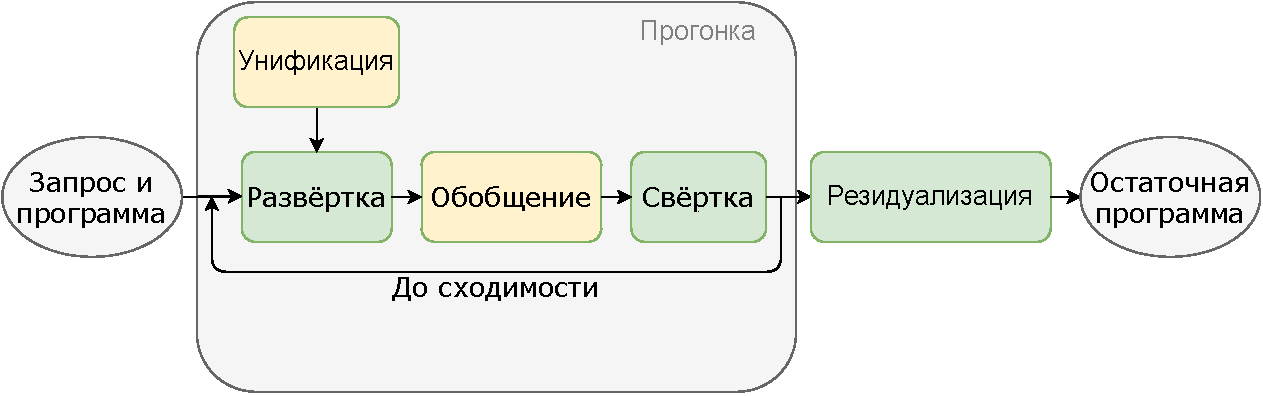
\includegraphics[scale=0.55]{scompflow.pdf}
\caption{
    Схема алгоритма суперкомпиляции\\
}
\label{fig:scomp}
\end{figure}
{\footnotesize
\begin{tabular}{l}

\includegraphics[scale=0.4]{orange.pdf} --- библиотека по специализации miniKanren c дополнениями\\

\includegraphics[scale=0.4]{green.pdf} --- собственная разработка
\end{tabular}
}

%В процессе суперкомпиляции строится корневой ориентированный граф, описывающий историю символьного исполнения,
%из которого извлекается \emph{остаточная} программа --- специализированная версия исходной.

\end{frame}

\begin{frame}{Результаты задачи}
\begin{itemize}
\item Реализован базовый алгоритм суперкомпиляции.
\begin{itemize}
\item Используемый алгоритм обобщения основан на алгоритме для конъюнктивной частичной дедукции,
      для которого доказана терминируемость.
\end{itemize}
\item Придуман и реализован алгоритм построения оптимизированной программы по графу суперкомпиляции.
\end{itemize}
\end{frame}

\begin{frame}{Улучшение суперкомпиляции для $\mu$Kanren}
\begin{block}{Проблемы}
\begin{itemize}
%\item Свёртка только на родителей: повторные символьные вычисления.
\item Повторение символьных вычислений.\\
%Решается кэшированием.
\item Обобщение только на родителей: слишком много вычислений перед свёрткой.
\item Обобщение вверх: в некоторых случаях нет эффекта от того, что часть входных данных известна.
\item Тривиальный шаг прогонки порождает слишком много ветвей исполнения.\\
%Решение: исследовать способы реализации шага прогонки.
\item Нет способа эффективно сообщить $\mu$Kanren, что можно прервать вычисление, из-за
чего суперкомпилятору приходится вычислять заведомо избыточные ветви.\\
%Решение: расширить язык оператором неравенства из miniKanren.
\end{itemize}
\end{block}
\end{frame}
%%%%%%%%%%%%%%%%%%%%%%%%%%%%%%%%%%%%%%%%%%%%%%%%%%%
% Базовый алгоритм:
% * ренейминг на родителей
% * обобщение на родителей
% * обобщение вверх
%%%%%%%%%%%%%%%%%%%%%%%%%%%%%%%%%%%%%%%%%%%%%%%%%%%
%\begin{frame}{Улучшение суперкомпиляции для $\mu$Kanren}
%\begin{block}{Варианты улучшения}
%\begin{itemize}
%\item Поиск более подходящей стратегии развёртывания для шага прогонки.
%\item Частичный или полный отказ от обобщения вверх.
%\item Обобщение на уже вычисленные вершины.
%\end{itemize}
%\end{block}
%\end{frame}

\begin{frame}{Улучшение суперкомпиляции для $\mu$Kanren}{Стратегии вычисления выражения на шаге прогонки}

\begin{block}{}
Разные стратегии вычисления выявляют разные возможности для оптимизации.
\end{block}

\begin{itemize}
\item Всегда вычислять первый вызов за шаг.
\item Вычислять все вызовы за шаг. % получая при этом все возможные способы развития сюжета
\item Последовательно вычислять вызовы.
\item В первую очередь вычислять не рекурсивные вызовы.
\item В первую очередь вычислять рекурсивные вызовы.
\item В первую очередь вычислять выражения с минимальным числом ветвлений.
\item В первую очередь вычислять выражения с максимальным числом ветвлений.
\end{itemize}

% В шаг суперкомпиляции приходит запрос, который представляет собой конъюнкцию вызовов реляционных отношений.
% Однако порядок развёртывания конъюнктов может быть разным: в зависимости от структуры конъюнкта
% разный порядок может приводить к разным результатам, поэтому нужно придумать что-нибудь хитрое:
% что не приводит к большому разростанию количества ветвей, но и даёт хорошие результаты.
\end{frame}

%\begin{frame}{Улучшение суперкомпиляции для $\mu$Kanren}{Расширение языка неравенставами}
%\begin{block}{Неравенства (англ. disequality constraints)}
%В miniKanren есть оператор неравенства ($\not\equiv$), который успешно выполняется в случае
%неуспешной унификация термов.
%\end{block}
%\end{frame}

\begin{frame}{Результаты задачи}
\begin{itemize}
\item Применены подходы по улучшению алгоритма суперкомпиляции.
\begin{itemize}
\item Добавлено кэширование.
\item Добавлено обобщение на все вычисленные вершины.
\item Добавлена возможность частично или полностью исключить обобщение вверх.
\item Проанализированы стратегии развёртывания.
\end{itemize}
\item Расширение библиотеки для специализации неравенствами.
\end{itemize}
\end{frame}

%%%%%%%%%%%%%%%%%%%%%%%%%%%%%%%%%%%%%%%%%%%%%%%%%%%
%
%%%%%%%%%%%%%%%%%%%%%%%%%%%%%%%%%%%%%%%%%%%%%%%%%%%
\begin{frame}{Тестирование}

{\bf Сценарий тестирования:}
\begin{enumerate}
\item Cпециализация реляционной программы.
\item Трансляция остаточной программы в DSL языка реализации miniKanren.
\item Запуск программы.
\item Сравнение времени исполнения с CPD и оригинальной программой.
\end{enumerate}

\begin{description}[leftmargin=!]
\item[Реализация miniKanren:] проект OCanren\footnote{\url{https://github.com/JetBrains-Research/OCanren}}\\
\item[Реализация CPD для miniKanren:] проект uKanren\_transformations\footnote{\url{https://github.com/kajigor/uKanren_transformations/}}
\item[Реализация CPD для Prolog:] проект ECCE\footnote{\url{https://github.com/leuschel/ecce}}
\item[Платформа:] Intel Core i5-6200U CPU, 2.30GHz, DDR4, 12GiB.
\end{description}
\end{frame}

%%%%%%%%%%%%%%%%%%%%%%%%%%%%%%%%%%%%%%%%%%%%%%%%%%%
%
%%%%%%%%%%%%%%%%%%%%%%%%%%%%%%%%%%%%%%%%%%%%%%%%%%%
\begin{frame}{Тестирование}
{\bf Программы для тестирования}
\begin{description}
\item[sort]Алгоритм реляционной сортировки.\\
      % Запрос: $\text{sort}^o$ xs ys.
      Запрос : сортировка случайного списка длины 50
\item[isPath] Проверка принадлежности пути графу.\\
      % Запрос: $\text{isPath}^o$ p g true.
      Запрос: поиск  произвольного пути длины 10, принадлежащих графу c 21 вершиной и 50 рёбрами.
\item[logint] Реляционный интерпретатор формул логики высказываний.\\
      Запрос: поиск 1000 истинных формул в данной подстановке.
      % Запрос: $\text{logint}^o$ s q true.
\item[lam] Реляционный интерпретатор лямбда-выражений.\\
      % Запрос: $\text{lam}^o$ q q.
      Запрос: поиск n термов в указаной форме.
% \item Реляционный алгоритм вывода типов для просто типизированного лямбда-исчисления.
%\item[a] Реляционный интерпретатор подмножества Scheme.
\end{description}
\end{frame}
%%%%%%%%%%%%%%%%%%%%%%%%%%%%%%%%%%%%%%%%%%%%%%%%%%%
%
%%%%%%%%%%%%%%%%%%%%%%%%%%%%%%%%%%%%%%%%%%%%%%%%%%%
\begin{frame}{Результаты тестирования}{Базовый суперкомпилятор}
% \begin{block}{Запуск в прямом направлении}
% \begin{itemize}
% \item Генерация подстановки по формуле: CPD работает в 50 раз быстрее, суперкомпилятор -- в 25 раз.
% \item Поиск 500 путей произвольной длины в графе $K_{10}$: CPD работает в 1.5 раза быстрее, суперкомпилятор -- в 2 раза.
% \end{itemize}
% \end{block}
% \begin{block}{Запуск в обратном направлении}
% \begin{itemize}
% \item Генерация формул: CPD работает в 12 медленнее, суперкомпилятор -- в 5 раз быстрее.
% \item Поиск пути заданной длины (15) в графе $K_{10}$: CPD работает в 2 раза медленнее, суперкомпилятор -- в 20 раз быстрее.
% \end{itemize}
% \end{block}

\begin{table}
\center
\begin{tabular}{|c|c|c|c|c|}
\hline
{\it Параметр} & {\it Оригинал} & {\it Ecce }  & {\it Cpd} & {\it СК} \\ \hline

\rowcolor{black!10}
{\bf sort} & \multicolumn{4}{|l|}{случайный список длины 50 } \\ \hline
         & 8.42     & 12.28 & 13.2 & 0.26    \\ \hline

\rowcolor{black!10}
{\bf isPath} & \multicolumn{4}{|l|}{произвольный путь длины 10} \\ \hline
граф 1 & > 300    & 9     & 10   & 0.25   \\ 
граф 2 &          & 2.7   & 2.8  & 0.1    \\
% граф 3 &          & 0.35  & 0.4  & 0.006  \\
\hline

\rowcolor{black!10}
{\bf logint} & \multicolumn{4}{|l|}{размер подстановки} \\ \hline
0 & > 300    & 0.17  & 2.7  & 0.09    \\
1 &          & 0.09  & 1.7  & 0.07    \\
%2 &         & 0.8   & 0.5 & 0.3      \\
\hline

\rowcolor{black!10}
{\bf lam} & \multicolumn{4}{|l|}{редуцируются} \\ \hline
10 термов к себе    & 0.17     & 0.001 & 0.008 & 0.002  \\
50 термов к себе    & > 300    & 2.98  & 4.32  & 1.79   \\
1000 термов к const & 1.01     & 0.126 & 0.263 & 0.274  \\
\hline
\end{tabular}
\end{table}

\end{frame}

\begin{frame}{Результаты тестирования}{Улучшения}
%\begin{itemize}
%\item Смена стратегии вычисления в базовом суперкомпиляторе:
%\begin{itemize}
%\item Не ухудшило время работы на логическом интерпретаторе.
%\item Поиск всех путей: в 5 раз быстрее. 
%\item Поиск пути заданной длины: в 25 раз быстрее.
%\end{itemize}
%
%\item + обобщение на все вычисленные вершины:
%\begin{itemize}
%\item Поиск пути заданной длины: в 40 раз быстрее (против 20).
%\item Поиск путей произвольной длины: в 5 раз быстрее (против 2).
%\item Генерация подстановки по формуле: в 40 раз (против 25).
%\end{itemize}
%
%\end{itemize}
%
%{\bf TODO:} обработка и анализ остальных тестов.
\end{frame}


%%%%%%%%%%%%%%%%%%%%%%%%%%%%%%%%%%%%%%%%%%%%%%%%%%%
%
%%%%%%%%%%%%%%%%%%%%%%%%%%%%%%%%%%%%%%%%%%%%%%%%%%%
\begin{frame}{Результаты работы}
  \begin{itemize}
  \item Реализован и протестирован суперкомпилятор для задачи специализации.
  \item Применены подходы по улучшению качества суперкомпиляции для задачи специализации.
  \item Добавлены неравенства в библиотеку по специализации.
  \item Реализованы реляционные интерпретаторы для тестирования.
  \item Проведено тестирование и анализ результатов.
  \item Исправление багов библиотеки для специализации.
  \end{itemize}
\end{frame}

\begin{frame}{Спасибо за внимание!}
\begin{itemize}
\item Работа будет представлена во второй половине мая на воркшопе по трендам логического программирования TEASE-LP.
\item Ссылка на репозиторий: \url{https://github.com/RehMaar/uKanren-spec}
\end{itemize}
\end{frame}


% Доп. слайды.
% Пример специализации.

\end{document} 
